\chapter{Water exchanges between Raven and MODFLOW}\label{ch:c4}
Raven and MODFLOW exchange water in eight ways (Table~\ref{tab:exchanges}). Each section below explains what the exchange represents and gives its equations. It then says what Raven does with the
result, which safeguards keep the water accounts exact, which inputs control it, where to see it in the outputs, and gives
a worked example.

\begin{plain}
Water crosses between the two models in eight places. The two main ones are \emph{recharge} --- water soaking down from
Raven's soil to the water table --- and \emph{seepage} --- groundwater coming back up where the water table reaches the ground.
Rivers, lakes and reservoirs, wetlands, wells and evaporation from a shallow water table make up the rest. For each one this
chapter gives the formula, a worked example with numbers, and the checks that make sure no water is created or lost on the
way.
\end{plain}
\begin{table}[!htbp]\centering
\caption{The eight exchanges between Raven and MODFLOW.}\label{tab:exchanges}\small
\begin{tabular}{lllll}\toprule\hdr
Exchange & Direction & MODFLOW package & Raven side & Section\\\midrule
Recharge & Raven $\to$ aquifer & RCH & \cmd{GROUNDWATER} & \ref{ch:recharge}\\
Seepage & aquifer $\to$ Raven & DRN & lowest soil layer & \ref{ch:seepage}\\
Rivers & both & RIV & reach inflow & \ref{ch:rivers}\\
Water-table ET & aquifer $\to$ air & EVT & unmet PET & \ref{ch:et}\\
Wetlands, lakes & both & RIV & HRU store & \ref{ch:stores}\\
Reservoirs & both & WEL & reservoir seepage & \ref{ch:reservoirs}\\
Wells & out (or in) & WEL & time series & \ref{ch:wells}\\
Boundaries & both & GHB, CHD & time series & \ref{ch:wells}\\\bottomrule
\end{tabular}\end{table}
\begin{figure}[!htbp]\centering
\begin{tikzpicture}[x=1cm,y=1cm,lab/.style={font=\scriptsize,align=center},ar/.style={-{Stealth[length=2mm]},thick}]
\fill[orange!20] (0,0.8) rectangle (14,3.2); \fill[black!12] (0,0) rectangle (14,0.8);
\draw[thick,brown!60!black] (0,3.6) -- (2.8,3.6) -- (3.2,3.0) -- (4.2,3.0) -- (4.6,3.6) -- (7.6,3.6) -- (7.9,3.3) -- (9.3,3.3) -- (9.6,3.6) -- (14,3.6);
\fill[blue!25] (3.05,3.4) -- (4.35,3.4) -- (4.2,3.0) -- (3.2,3.0) -- cycle; \node[lab] at (3.7,4.05) {river};
\fill[cyan!20] (7.75,3.5) -- (9.45,3.5) -- (9.3,3.3) -- (7.9,3.3) -- cycle; \node[lab] at (8.6,4.05) {wetland / lake};
\draw[dashed,blue!70!black,thick] (0,3.3) .. controls (2,3.2) and (2.8,3.05) .. (3.7,3.1) .. controls (5,3.2) and (7,3.45) .. (8.6,3.5) .. controls (10,3.5) and (12,3.1) .. (14,2.9);
\node[lab,blue!70!black,anchor=west] at (1.25,2.8) {water table};
\draw[ar,teal!70!black] (1.0,4.6) -- node[lab,right]{recharge} (1.0,3.35);
\draw[ar,teal!70!black] (6.1,3.45) -- node[lab,right]{seepage} (6.1,4.5);
\draw[ar,blue!70!black,<->] (3.7,2.95) -- node[lab,right]{river exchange} (3.7,2.2);
\draw[ar,cyan!60!black,<->] (8.6,3.25) -- node[lab,right]{store exchange} (8.6,2.4);
\draw[ar,green!50!black] (10.9,3.25) -- node[lab,right]{water-table ET} (10.9,4.5);
\draw[thick] (13.2,4.7) -- (13.2,1.4); \draw[ar,red!70!black] (13.2,1.8) -- node[lab,left,pos=0.9]{well} (13.2,4.8);
\draw[ar,purple!70!black,<->] (0.1,1.7) -- node[lab,above]{GHB / CHD} (1.6,1.7);
\node[lab] at (7,1.6) {aquifer (MODFLOW)}; \node[lab] at (7,0.4) {bedrock};
\end{tikzpicture}
\caption{The exchanges between Raven (above the water table) and MODFLOW (below). Reservoir seepage works like the store
exchange, through Raven's reservoir seepage law.}\label{fig:allexch}
\end{figure}

\section{Recharge: from Raven to the water table}\label{ch:recharge}
\subsection{Where recharge comes from}
Any Raven process that moves water into \cmd{GROUNDWATER} in a coupled HRU produces recharge --- no special process is
needed. For example, in the Liard model the percolation from the fast reservoir is sent to \cmd{GROUNDWATER} for coupled
HRUs:
\par\noindent\begin{minipage}{\linewidth}
\begin{lstlisting}
:Percolation PERC_CONSTANT FAST_RESERVOIR GROUNDWATER
  :-->Conditional HRU_GROUP IS AquiferHRUs
\end{lstlisting}
\end{minipage}\par\smallskip
At the end of a day, the \cmd{GROUNDWATER} store of HRU $k$ holds $r_k$ mm; this is the recharge of that day. Raven
counts it as water leaving Raven (its balance, Section~\ref{ch:balance}), and it is empty again at the start of the
next day.

\subsection{Volume of recharge}
\begin{equation}
V_k=\frac{r_k}{1000}\,A_k \quad[\mathrm{m}^3],
\end{equation}
with $A_k$ the HRU area from the \cmd{.rvh} file in m$^2$.

\subsection{Optional recharge delay}
Where the water table is deep, water takes time to cross the unsaturated zone. With the aquifer profile parameter \cmd{RECHARGE\_DELAY}~$\tau>0$ (Section~\ref{app:profile})
(days) the recharge passes through a linear reservoir $S_k$ before reaching the water table:
\begin{equation}
S_k^{*}=S_k^{n}+V_k,\qquad V_k^{\mathrm{out}}=S_k^{*}\left(1-e^{-\dt/\tau}\right),\qquad S_k^{n+1}=S_k^{*}-V_k^{\mathrm{out}} .
\end{equation}
With $\tau=0$ the delay is off and $V_k^{\mathrm{out}}=V_k$. The delay store is reported in \cmd{GWBudget.csv}, saved in
\cmd{solution.rvc} (\cmd{:GWRechargeStore}) and read back on hotstart.
\begin{example}[: recharge delay]
$\tau=60$ d, $\dt=1$ d: each day $1-e^{-1/60}=1.65\%$ of the store is released. A single 1\,000 m$^3$ pulse reaches the
water table as 16.5 m$^3$ on the first day, then less each day; after 60 days 63\% of it has arrived
(Figure~\ref{fig:curves}a).
\end{example}

\subsection{Spreading recharge over the cells}
The released volume is shared among the HRU's cells in proportion to overlap. Cells whose top cell holds a fixed head
(Section~\ref{ch:wells}) are skipped, because MODFLOW ignores recharge there:
\begin{equation}
Q^{\mathrm{rch}}_i=\sum_{k\in\mathcal{K}}\frac{V_k^{\mathrm{out}}}{\dt}\,\frac{A_{k,i}}{\sum_{j\notin\mathcal{C}}A_{k,j}}
\quad[\mathrm{m}^3/\mathrm{d}],\qquad R_i=\frac{Q^{\mathrm{rch}}_i}{\Delta^2}\quad[\mathrm{m/d}],
\end{equation}
where $\mathcal{C}$ are the fixed-head columns. $R_i$ is the recharge rate given to MODFLOW's RCH package, applied to the top cell of the column
(the top layer of an active column is always active). The fractions for one HRU always add up to one, so exactly $V_k^{\mathrm{out}}$
enters MODFLOW. If an HRU lies entirely on fixed-head cells, its recharge passes to that boundary and is reported in the
column \emph{recharge onto CHD cells}.
\begin{example}[: spreading recharge]
The 10 km$^2$ HRU of the Section~\ref{ch:grid} example receives 2 mm in a day: $V=0.002\times10^7=20\,000$ m$^3$. The three
cells get 8\,000, 7\,000 and 5\,000 m$^3$/d; for 4 km$^2$ cells the recharge rates are 2.0, 1.75 and 1.25 mm/d
(plus any recharge from other HRUs in the same cells).
\end{example}

\begin{figure}[!htbp]\centering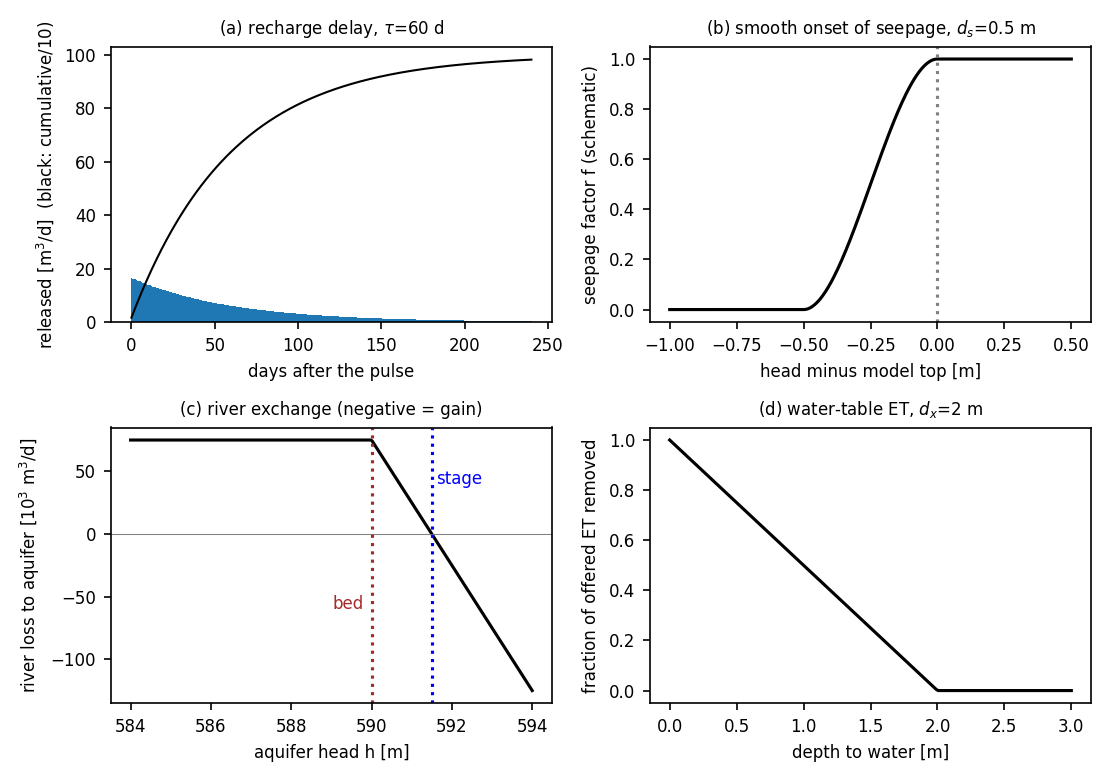
\includegraphics[width=\linewidth]{figures/fig_curves.png}
\caption{Response curves of four exchanges: (a) recharge delay reservoir after a 1\,000 m$^3$ pulse ($\tau=60$ d);
(b) seepage factor near the model top ($d_s=0.5$ m); (c) river flow against aquifer head; (d) water-table ET against
depth ($d_x=2$ m).}\label{fig:curves}\end{figure}

\begin{refcard}{recharge}
\textbf{Sources/sinks.} Moves water from \cmd{GROUNDWATER} of each coupled HRU to the aquifer (MODFLOW RCH package \cmd{RCH\_RAVEN}, top cell of each
active column), optionally through the recharge-delay store (internal to the coupling, saved in \cmd{solution.rvc}).\par\smallskip
\textbf{Constraints/notes.} In a coupled HRU \cmd{GROUNDWATER} is a pass-through: no Raven process may draw water from it (start-up error). Recharge is
never negative. The volume of each HRU is conserved exactly; recharge of HRUs lying wholly on fixed-head cells is reported
separately.\par\smallskip
\par\noindent\begin{minipage}{\linewidth}\textbf{Command syntax}
\begin{lstlisting}
# .rvi -- any process that moves water into GROUNDWATER in coupled HRUs, e.g.
:Percolation  PERC_CONSTANT  FAST_RESERVOIR  GROUNDWATER
  :-->Conditional HRU_GROUP IS AquiferHRUs
# .rvp -- optional recharge delay, per aquifer profile
:AquiferProfileParameters
  :Attributes,     RECHARGE_DELAY
  :Units,          d
  VALLEY_ALLUVIUM, 30.0
:EndAquiferProfileParameters
\end{lstlisting}
\end{minipage}\par\smallskip
\par\noindent\begin{minipage}{\linewidth}\textbf{Parameters}\par\smallskip
\begin{tabular}{>{\raggedright\arraybackslash}P{0.09\linewidth}>{\raggedright\arraybackslash}P{0.26\linewidth}>{\raggedright\arraybackslash}P{0.283\linewidth}>{\raggedright\arraybackslash}P{0.1\linewidth}>{\raggedright\arraybackslash}P{0.15\linewidth}}\toprule\hdr \hdr Symbol & Parameter & Class (where it is set) & Units & Reference\\\midrule
$r_k$ & \cmd{GROUNDWATER} & Raven state variable of HRU $k$ (filled by the chosen process) & mm & Raven state var.\\
$A_k$ & \cmd{AREA} & HRU (\cmd{:HRUs}, \cmd{.rvh}) & km$^2$ & Raven manual\\
$\tau$ & \cmd{RECHARGE\_DELAY} & aquifer profile (\cmd{:AquiferProfile\allowbreak Parameters}) & d & Sec.~\ref{app:profile}\\
$A_{k,i}$ & overlap area & computed from \cmd{:HRUGeometry} (\cmd{.rvg}) & m$^2$ & Sec.~\ref{ch:grid}\\
$\Delta$ & \cmd{:GridCellSize} & \cmd{.rvg} option & m & Sec.~\ref{app:commands}\\
\bottomrule\end{tabular}\end{minipage}\par\smallskip
\textbf{Outputs.} \cmd{GWBudget.csv}: \emph{Raven recharge}, \emph{MF6 recharge}, \emph{recharge delay storage}, \emph{recharge onto CHD cells};
Raven's \cmd{GROUNDWATER} storage shows each day's recharge (mm) of every HRU.
\end{refcard}

\subsection{Common questions}
\textit{Can recharge be negative?} Only if a Raven process removes water from \cmd{GROUNDWATER}, which is forbidden in coupled
HRUs; recharge is therefore never negative. \textit{Does recharge depend on the water table?} Not directly --- Raven decides
it. If the water table reaches the surface, the extra water returns immediately as seepage (Section~\ref{ch:seepage}), which
acts as ``rejected recharge''.

\section{Seepage: groundwater returning to the surface}\label{ch:seepage}
Where the water table reaches the land surface, groundwater flows out: springs, wet meadows, seepage faces. Every active
column has a drain (MODFLOW's DRN package) at the model top that removes water whenever the water table is close to
the top, and hands it back to Raven.

\subsection{Equation}
\begin{equation}
Q^{\mathrm{seep}}_i=C^{\mathrm{drn}}_i\;f\!\left(h_i\right)\left(h_i-z_{\mathrm{top},i}+d_s\right)\ \text{ for } h_i>z_{\mathrm{top},i}-d_s,
\qquad C^{\mathrm{drn}}_i=L_s\,\Delta^2 ,
\end{equation}
where $L_s$ [1/d] is the aquifer profile parameter \cmd{SEEPAGE\_LEAKANCE} and $d_s$ [m] the aquifer profile parameter \cmd{SEEPAGE\_SMOOTHING\_DEPTH} (Section~\ref{app:profile}).
The factor $f$ rises smoothly from 0 at $d_s$ below the top to 1 at the top (Figure~\ref{fig:curves}b). Where the top cell is
thinner than $d_s$, $d_s$ is limited to its thickness (MODFLOW does not accept a smoothing interval below the cell). Without this
smoothing the drain would switch on abruptly, which makes the Newton iterations harder; with it, seepage starts gently
as the water table approaches the surface.

\subsection{Back to Raven}
Each column's seepage is shared among the HRUs above it by overlap:
\begin{equation}
V^{\mathrm{ret}}_k=\sum_i Q^{\mathrm{seep}}_i\,\dt\,\frac{A_{k,i}}{\sum_{m}A_{m,i}},
\end{equation}
and added to the Raven store \cmd{:SeepageReturnTo} of HRU $k$ (default: the lowest soil layer) as
$1000\,V^{\mathrm{ret}}_k/A_k$ mm. HRUs without soil layers (lake, glacier or rock profiles) receive it in
\cmd{SURFACE\_WATER} instead. From there Raven's own processes take it on --- for example, the baseflow process of the
lowest soil layer carries it to the river.
\begin{example}[: seepage]
A 4 km$^2$ cell with $L_s=1$ d$^{-1}$ has $C=4\times10^6$ m$^2$/d. With the water table 0.1 m above the top and the
factor $f=1$, seepage is $4\times10^6\times(0.1+0.5)\approx2.4\times10^6$ m$^3$/d --- a large number, which is why in
practice the water table settles very close to the surface wherever the aquifer is full: the drain is a strong outlet.
\end{example}

\begin{refcard}{seepage}
\textbf{Sources/sinks.} Moves water from the aquifer (MODFLOW DRN package \cmd{DRN\_RAVEN} at the model top of every active column) to the Raven
store named by \cmd{:SeepageReturnTo} in each overlapping HRU --- by default the lowest soil layer \cmd{SOIL[$m$]}, and
\cmd{SURFACE\_WATER} for HRUs without soil layers.\par\smallskip
\textbf{Constraints/notes.} Seepage occurs only when the head is within $d_s$ of the model top; it is returned to Raven by overlap, exactly. In a step that
does not converge, seepage (with river gains and store discharge) is limited to the step's inflow.\par\smallskip
\par\noindent\begin{minipage}{\linewidth}\textbf{Command syntax}
\begin{lstlisting}
# .rvp
:AquiferProfileParameters
  :Attributes,     SEEPAGE_LEAKANCE, SEEPAGE_SMOOTHING_DEPTH, SOIL_ZONE_DEPTH
  :Units,          1/d,              m,                       m
  VALLEY_ALLUVIUM, 1.0,              0.5,                     0.0
:EndAquiferProfileParameters
# .rvg -- optional
:SeepageReturnTo  SOIL[2]
\end{lstlisting}
\end{minipage}\par\smallskip
\par\noindent\begin{minipage}{\linewidth}\textbf{Parameters}\par\smallskip
\begin{tabular}{>{\raggedright\arraybackslash}P{0.09\linewidth}>{\raggedright\arraybackslash}P{0.26\linewidth}>{\raggedright\arraybackslash}P{0.283\linewidth}>{\raggedright\arraybackslash}P{0.1\linewidth}>{\raggedright\arraybackslash}P{0.15\linewidth}}\toprule\hdr \hdr Symbol & Parameter & Class (where it is set) & Units & Reference\\\midrule
$L_s$ & \cmd{SEEPAGE\_LEAKANCE} & aquifer profile & 1/d & Sec.~\ref{app:profile}\\
$d_s$ & \cmd{SEEPAGE\_SMOOTHING\_DEPTH} & aquifer profile & m & Sec.~\ref{app:profile}\\
$z_{\mathrm{top}}$ & land surface $-$ \cmd{SOIL\_ZONE\_DEPTH} & \cmd{:LandSurface} (\cmd{.rvg}); aquifer profile & m & Sec.~\ref{app:profile}\\
-- & \cmd{:SeepageReturnTo} & \cmd{.rvg} option (a Raven storage state variable) & -- & Sec.~\ref{app:commands}\\
\bottomrule\end{tabular}\end{minipage}\par\smallskip
\textbf{Outputs.} \cmd{GWBudget.csv}: \emph{seepage to Raven} and \emph{returned to Raven} (equal); the receiving store in Raven's outputs.
\end{refcard}

\subsection{Choosing the leakance}
A large leakance makes the drain a strong outlet: the water table then stays within a few centimetres of the surface wherever
the aquifer is full, and seepage follows recharge closely. A small leakance lets the water table rise above the surface
(ponding in the model's sense) and delays seepage. Values of 0.1--10 d$^{-1}$ cover most cases; 1 d$^{-1}$ is the default.

\section{Rivers}\label{ch:rivers}
Rivers exchange water with the aquifer in both directions: a \emph{gaining} river receives groundwater (baseflow); a
\emph{losing} river leaks into the aquifer. The coupling uses MODFLOW's RIV package in every cell crossed by a river line
(\cmd{:RiverGeometry}), with river levels taken from Raven's own river routing.

\subsection{River cells}
River lines (GeoJSON, lon/lat) are cut into short pieces (1/20 of a cell) and each piece is assigned to the cell under its
midpoint. For each subbasin $p$ and cell $i$ Raven records the river length $L_{p,i}$ and the lowest DEM value along the
line in that cell. The subbasin of a piece comes from an ID field in the GeoJSON, or, if none is given, from the subbasin
of the dominant HRU of the cell.

\subsection{Riverbed elevation and river level}
The DEM usually records the water surface or floodplain along a river, so the bed lies one bankfull depth below it:
\begin{equation}
z_{\mathrm{bed}}=\min_{\text{line in cell}}z_{\mathrm{DEM}}-d_{\mathrm{bf},p},
\end{equation}
where $d_{\mathrm{bf},p}$ is the depth of Raven's channel at its reference flow (or the value of \cmd{:RiverBedDepth});
$z_{\mathrm{bed}}$ is also never placed above the model top.
The bed is never placed above the model top nor below the column: if it would lie below every active cell, it is set
0.1 m above the lowest active cell bottom. The river cell is placed in the highest active layer whose bottom is below the
bed. Each day the river level (\emph{stage}) is
\begin{equation}
s=\min\!\left(z_{\mathrm{bed}}+d_p(t),\ z_{\mathrm{land},i}\right),
\end{equation}
with $d_p(t)$ Raven's channel depth at the start of the day. Above bankfull the extra water is on the floodplain, which
is not part of this exchange, so the stage is capped at the land surface.

\subsection{Exchange equation}
\begin{equation}
q^{\mathrm{riv}}=\begin{cases}C^{\mathrm{riv}}\left(s-h\right) & h>z_{\mathrm{bed}},\\
C^{\mathrm{riv}}\left(s-z_{\mathrm{bed}}\right) & h\le z_{\mathrm{bed}},\end{cases}
\qquad C^{\mathrm{riv}}=\frac{K_b\,W_p(t)\,L_{p,i}}{M_b},
\end{equation}
with $K_b$ [m/d] the riverbed conductivity (aquifer profile parameter \cmd{RIVERBED\_K}), $M_b$ [m] its thickness (aquifer profile parameter \cmd{RIVERBED\_THICKNESS}; Section~\ref{app:profile}) and $W_p(t)$
Raven's channel top width. Positive $q$ is a losing river. When the water table drops below the bed, the river is
\emph{disconnected}: it leaks at a constant maximum rate, whatever the depth of the water table
(Figure~\ref{fig:curves}c).

\begin{figure}[!htbp]\centering
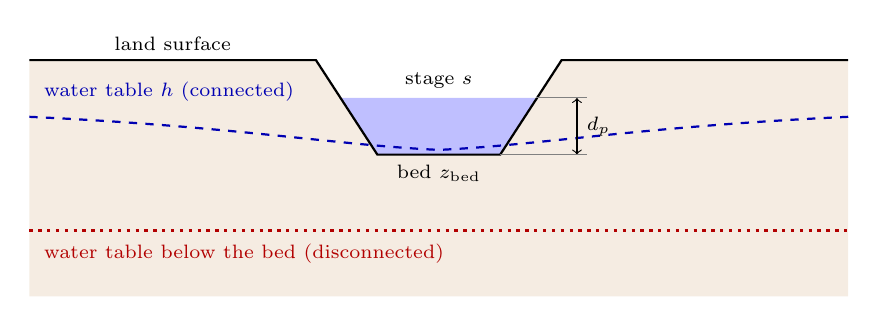
\begin{tikzpicture}[x=1.3cm,y=1.2cm,lab/.style={font=\scriptsize}]
\fill[brown!15] (-4,0) -- (4,0) -- (4,2.5) -- (1.2,2.5) -- (0.6,1.5) -- (-0.6,1.5) -- (-1.2,2.5) -- (-4,2.5) -- cycle;
\fill[blue!25] (-0.95,2.1) -- (0.95,2.1) -- (0.6,1.5) -- (-0.6,1.5) -- cycle;
\draw[thick] (-4,2.5) -- (-1.2,2.5) -- (-0.6,1.5) -- (0.6,1.5) -- (1.2,2.5) -- (4,2.5);
\draw[dashed,blue!70!black,thick] (-4,1.9) .. controls (-2,1.8) and (-1,1.6) .. (0,1.55) .. controls (1,1.6) and (2,1.8) .. (4,1.9);
\node[lab,blue!70!black,anchor=west] at (-3.95,2.17) {water table $h$ (connected)};
\draw[dotted,red!70!black,very thick] (-4,0.7) -- (4,0.7); \node[lab,red!70!black,anchor=west] at (-3.95,0.45) {water table below the bed (disconnected)};
\draw[<->] (1.35,1.5) -- (1.35,2.1); \node[lab,right] at (1.35,1.8) {$d_p$};
\draw[gray,thin] (0.6,1.5) -- (1.45,1.5); \draw[gray,thin] (0.95,2.1) -- (1.45,2.1);
\node[lab] at (0,2.28) {stage $s$}; \node[lab] at (0,1.3) {bed $z_{\mathrm{bed}}$};
\node[lab,anchor=south] at (-2.6,2.5) {land surface};
\end{tikzpicture}
\caption{River cell: stage $s$ = bed + Raven channel depth. With the water table above the bed, flow is $C(s-h)$ (either
direction); below the bed the river is disconnected and leaks at $C(s-z_{\mathrm{bed}})$.}\label{fig:river}
\end{figure}

\subsection{Never taking water the river does not have}
A losing river cannot give more than it carries. The conductance is therefore limited each day so that the largest
possible loss --- the disconnected rate $C(s-z_{\mathrm{bed}})$ --- is no more than the cell's share (by river length) of
the flow in the channel reach at the start of the day (the channel flow, upstream of any reservoir at the subbasin outlet):
\begin{equation}
C^{\mathrm{riv}}\le\frac{Q^{\mathrm{out}}_p\,(L_{p,i}/L_p)}{s-z_{\mathrm{bed}}},
\end{equation}
with $Q^{\mathrm{out}}_p$ in m$^3$/d and $L_p$ the subbasin's total river length on active cells. (Using the reservoir
release instead would cut off every river cell above a lake whenever the lake is not spilling.) Rivers of disabled
subbasins get no river cells.

\subsection{Back to Raven's rivers}
For each subbasin the net aquifer discharge is $G_p=-\sum_i q^{\mathrm{riv}}_{p,i}$ [m$^3$/d]. A gain is added to the
subbasin's in-catchment inflow for the day (so it passes Raven's catchment routing like other runoff). A loss is taken
first from that in-catchment inflow and then, inside Raven's routing loop, from the flow entering the reach from
upstream. A loss that still cannot be supplied in the day --- rare, because of the limit above --- is \emph{carried} to the
next day and taken from the river first thing then, so no water is created:
\begin{equation}
V^{\mathrm{applied}}_{p,n}=G_{p,n}\,\dt-K_{p,n-1}+K_{p,n},
\end{equation}
where $K_{p,n}$ [m$^3$] is the loss carried out of day $n$. Summed over a run, the water applied to Raven equals MODFLOW's net
river exchange minus whatever is still carried at the end (written to \cmd{solution.rvc} as \cmd{:GWRiverLossCarry} and
taken on the first day of a restart).
\begin{example}[: river exchange]
$K_b=0.5$ m/d, $M_b=1$ m, width 40 m, 2\,500 m of river in the cell: $C=0.5\times40\times2\,500/1=50\,000$ m$^2$/d. Bed
590 m, depth 1.5 m, stage 591.5 m. Water table at 590.8 m: $q=50\,000\times0.7=35\,000$ m$^3$/d lost to the aquifer.
Water table at 592.0 m: $q=-25\,000$ m$^3$/d, a gain for the river. Water table at 585 m (below the bed): the river
leaks $50\,000\times1.5=75\,000$ m$^3$/d.
\end{example}

\begin{refcard}{rivers}
\textbf{Sources/sinks.} Exchanges water in both directions between the aquifer (MODFLOW RIV package \cmd{RIV\_RAVEN} in every river cell) and Raven's
reaches: gains are added to the subbasin's in-catchment inflow; losses are taken from it and then from the reach inflow.\par\smallskip
\textbf{Constraints/notes.} The conductance is limited by the channel flow at the start of the step; a loss that cannot be supplied is carried to the next
step. The stage never exceeds the land surface; the bed is never above the model top. Disabled subbasins get no river cells.\par\smallskip
\par\noindent\begin{minipage}{\linewidth}\textbf{Command syntax}
\begin{lstlisting}
# .rvg
:RiverGeometry  my_rivers.geojson  SubId     # river lines; subbasin ID field optional
:RiverBedDepth  REFERENCE_FLOW               # or a depth [m] below the DEM
# .rvp
:AquiferProfileParameters
  :Attributes,     RIVERBED_K, RIVERBED_THICKNESS
  :Units,          m/d,        m
  VALLEY_ALLUVIUM, 0.5,        1.0
:EndAquiferProfileParameters
\end{lstlisting}
\end{minipage}\par\smallskip
\par\noindent\begin{minipage}{\linewidth}\textbf{Parameters}\par\smallskip
\begin{tabular}{>{\raggedright\arraybackslash}P{0.09\linewidth}>{\raggedright\arraybackslash}P{0.26\linewidth}>{\raggedright\arraybackslash}P{0.283\linewidth}>{\raggedright\arraybackslash}P{0.1\linewidth}>{\raggedright\arraybackslash}P{0.15\linewidth}}\toprule\hdr \hdr Symbol & Parameter & Class (where it is set) & Units & Reference\\\midrule
$K_b$ & \cmd{RIVERBED\_K} & aquifer profile (of the column) & m/d & Sec.~\ref{app:profile}\\
$M_b$ & \cmd{RIVERBED\_THICKNESS} & aquifer profile & m & Sec.~\ref{app:profile}\\
$W_p$, $d_p$ & channel top width, depth & subbasin channel (\cmd{:ChannelProfile}, \cmd{.rvp}); Raven routing state & m & Raven manual\\
$d_{\mathrm{bf},p}$ & \cmd{:RiverBedDepth} or depth at \cmd{Q\_REFERENCE} & \cmd{.rvg} option; subbasin parameter (\cmd{.rvh}) & m & Sec.~\ref{app:commands}\\
$L_{p,i}$ & river length in a cell & computed from \cmd{:RiverGeometry} & m & Sec.~\ref{ch:rivers}\\
$Q^{\mathrm{out}}_p$ & channel flow & Raven routing state (subbasin) & m$^3$/s & Raven state var.\\
\bottomrule\end{tabular}\end{minipage}\par\smallskip
\textbf{Outputs.} \cmd{GWBudget.csv}: \emph{river leakage to aquifer}, \emph{aquifer discharge to rivers}, \emph{river exchange applied to Raven},
\emph{river loss carried to next step}; streamflow in \cmd{Hydrographs.csv} includes the exchange.
\end{refcard}

\subsection{Common questions}
\textit{Why is the stage from the start of the step?} Raven routes rivers after MODFLOW has solved; using the start-of-step
depth avoids iterating between the two models, and at daily steps the difference is small. \textit{What if a subbasin has no
channel?} Its depth and width are zero, so its conductance and stage give no exchange, and any groundwater reaching the surface
there leaves through the seepage drains. \textit{Headwater reaches with little flow} cannot lose much water, because the supply
limit scales the conductance with the reach outflow.

\section{Evaporation from a shallow water table}\label{ch:et}
Plants and bare soil can draw water directly from a water table close to the surface. With the aquifer profile parameter \cmd{EXTINCTION\_DEPTH} (Section~\ref{app:profile})
$d_x>0$, each active column gets MODFLOW's EVT package. Raven first satisfies evaporation from its own stores; only the
potential evaporation it could \emph{not} meet is offered to the water table:
\begin{equation}
E_i=\frac{1}{\Delta^2}\sum_kA_{k,i}\;\frac{\max\left(\mathrm{PET}_k\,\dt-\mathrm{AET}_k,\;0\right)}{1000\,\dt}\quad[\mathrm{m/d}],
\end{equation}
where $\mathrm{PET}_k$ [mm/d] is the HRU's potential evaporation and $\mathrm{AET}_k$ [mm] what Raven already evaporated
that day. Only HRUs whose own profile has an extinction depth contribute. The unmet demand of those HRUs in the cell (a volume) is spread over the whole cell area $\Delta^2$, because MODFLOW
multiplies the rate by the full cell area. The most MODFLOW can remove is then exactly that unmet volume, even where coupled
HRUs cover only part of the cell. MODFLOW removes
\begin{equation}
Q^{\mathrm{evt}}_i=E_i\,\Delta^2\;\min\!\left(1,\max\!\left(0,\;1-\frac{z_{\mathrm{land},i}-h_i}{d_x}\right)\right),
\end{equation}
the full rate when the water table is at the surface, falling linearly to zero at depth $d_x$ (Figure~\ref{fig:curves}d).
This water leaves the system as evaporation.
\begin{example}[: water-table ET]
Unmet PET 2 mm/d over a 4 km$^2$ cell fully covered by coupled HRUs, $d_x=2$ m, water table 0.5 m deep:
$Q=0.002\times4\times10^6\times(1-0.5/2)=6\,000$ m$^3$/d. If coupled HRUs covered only 1 km$^2$ of the cell, the unmet volume
would be 2\,000 m$^3$, $E=2\,000/4\times10^6=0.5$ mm/d over the cell, and $Q=1\,500$ m$^3$/d.
\end{example}

\begin{refcard}{water-table evaporation}
\textbf{Sources/sinks.} Moves water from the aquifer (MODFLOW EVT package \cmd{EVT\_RAVEN}, top cell) to the atmosphere. It leaves the system and is
not included in Raven's \cmd{AET}.\par\smallskip
\textbf{Constraints/notes.} Only HRUs whose aquifer profile has an extinction depth contribute; MODFLOW can never remove more than their unmet
evaporative demand; the rate falls linearly to zero at the extinction depth.\par\smallskip
\par\noindent\begin{minipage}{\linewidth}\textbf{Command syntax}
\begin{lstlisting}
# .rvp
:AquiferProfileParameters
  :Attributes,     EXTINCTION_DEPTH
  :Units,          m
  VALLEY_ALLUVIUM, 2.0
:EndAquiferProfileParameters
\end{lstlisting}
\end{minipage}\par\smallskip
\par\noindent\begin{minipage}{\linewidth}\textbf{Parameters}\par\smallskip
\begin{tabular}{>{\raggedright\arraybackslash}P{0.09\linewidth}>{\raggedright\arraybackslash}P{0.26\linewidth}>{\raggedright\arraybackslash}P{0.283\linewidth}>{\raggedright\arraybackslash}P{0.1\linewidth}>{\raggedright\arraybackslash}P{0.15\linewidth}}\toprule\hdr \hdr Symbol & Parameter & Class (where it is set) & Units & Reference\\\midrule
$d_x$ & \cmd{EXTINCTION\_DEPTH} & aquifer profile (0 = off) & m & Sec.~\ref{app:profile}\\
$\mathrm{PET}_k$ & potential evapotranspiration & Raven forcing function of HRU $k$ (\cmd{:Evaporation} method, \cmd{.rvi}) & mm/d & Raven manual\\
$\mathrm{AET}_k$ & \cmd{AET} & Raven state variable of HRU $k$ & mm & Raven state var.\\
\bottomrule\end{tabular}\end{minipage}\par\smallskip
\textbf{Outputs.} \cmd{GWBudget.csv}: \emph{water-table ET}. Total evaporation is Raven's AET plus this column.
\end{refcard}

\section{Wetlands and lakes held in Raven stores}\label{ch:stores}
Wetlands and small lakes are often represented in Raven by a store in their HRUs: \cmd{DEPRESSION} for wetlands, or
\cmd{LAKE\_STORAGE} for lakes. \cmd{:SurfaceWater\allowbreak Exchange SV group LEAKANCE L} connects such a store, in the HRUs of an HRU
group, to the aquifer below.

\subsection{The boundary}
In each column holding HRUs of the group, the exchange is a river-type boundary (MODFLOW RIV package) whose bed is the
model top and whose water level is the top plus the average depth of water in the store:
\begin{equation}
\bar s_i=\frac{\sum_kA_{k,i}\,s_k}{\sum_kA_{k,i}},\qquad h_b=z_{\mathrm{top},i}+\bar s_i,
\qquad q=\begin{cases}C\left(h_b-h\right) & h>z_{\mathrm{top},i},\\ C\,\bar s_i & h\le z_{\mathrm{top},i},\end{cases}
\end{equation}
with $s_k$ the store depth of HRU $k$ in metres ($1/1000$ of the store in mm). Positive $q$ is leakage from the store to
the aquifer; negative $q$ is groundwater feeding the store. Because leakage stops growing once the water table is below
the store's bed, it can never exceed $C\,\bar s_i$.

\subsection{Never draining more than the store holds}
The water available in a cell is the store's real volume, split among the HRU's cells by overlap and fixed at the start
of the day:
\begin{equation}
V_{k,i}=s_k\,A_k\,\frac{A_{k,i}}{\sum_jA_{k,j}},\qquad V_i=\sum_kV_{k,i} .
\end{equation}
The conductance is limited so that the largest possible leakage in the day is no more than this water:
\begin{equation}
C=\min\!\left(L\sum_kA_{k,i},\ \frac{V_i}{\dt\,\bar s_i}\right),\qquad C=0\ \text{when the stores are empty}.
\end{equation}
After MODFLOW solves, leakage is removed from each HRU's store in proportion to $V_{k,i}$, and groundwater discharge is
added in proportion to area. Because the shares come from the same fixed volumes used for the limit, no store can be
over-drawn and the volumes on both sides match exactly. A store of an HRU may be connected by only one
\cmd{:SurfaceWater\allowbreak Exchange}; Raven stops if two exchanges would draw on the same store. Groundwater that reaches the surface under an \emph{empty} store is
still returned to Raven by the seepage drain (Section~\ref{ch:seepage}).
\begin{example}[: wetland leakage]
Group HRUs cover 3 km$^2$ of a cell, $L=0.05$ d$^{-1}$: $C\le0.05\times3\times10^6=150\,000$ m$^2$/d. The wetland holds
20 mm ($\bar s=0.02$ m, $V=60\,000$ m$^3$ in this cell). The supply limit is $60\,000/(1\times0.02)=3\times10^6$ m$^2$/d, so
$C=150\,000$. With the water table 1 m below the top (disconnected), leakage is $150\,000\times0.02=3\,000$ m$^3$/d, i.e.\
1 mm/d over the 3 km$^2$.
\end{example}

\begin{refcard}{wetlands and lakes}
\textbf{Sources/sinks.} Exchanges water in both directions between a Raven storage state variable (e.g.\ \cmd{DEPRESSION}, \cmd{LAKE\_STORAGE},
\cmd{SOIL[0]}) of the HRUs in an HRU group and the aquifer (MODFLOW RIV package \cmd{SWX\_RAVEN}, top cell).\par\smallskip
\textbf{Constraints/notes.} The conductance is limited by the water stored, so a store can never be over-drawn; an empty store does not leak. A store of
an HRU may be connected by one exchange only.\par\smallskip
\par\noindent\begin{minipage}{\linewidth}\textbf{Command syntax}
\begin{lstlisting}
# .rvg
:SurfaceWaterExchange  DEPRESSION  WetlandHRUs  LEAKANCE 0.01
# .rvh
:HRUGroup WetlandHRUs
  101, 102, 157
:EndHRUGroup
\end{lstlisting}
\end{minipage}\par\smallskip
where \cmd{DEPRESSION} is the Raven store, \cmd{WetlandHRUs} an HRU group and 0.01 the leakance [1/d].
\par\smallskip\noindent\begin{minipage}{\linewidth}\textbf{Parameters}\par\smallskip
\begin{tabular}{>{\raggedright\arraybackslash}P{0.09\linewidth}>{\raggedright\arraybackslash}P{0.26\linewidth}>{\raggedright\arraybackslash}P{0.283\linewidth}>{\raggedright\arraybackslash}P{0.1\linewidth}>{\raggedright\arraybackslash}P{0.15\linewidth}}\toprule\hdr \hdr Symbol & Parameter & Class (where it is set) & Units & Reference\\\midrule
$L$ & \cmd{LEAKANCE} & \cmd{:SurfaceWater\allowbreak Exchange} argument (\cmd{.rvg}) & 1/d & Sec.~\ref{app:commands}\\
$s_k$ & store depth & Raven state variable (the named store) of HRU $k$ & mm & Raven state var.\\
-- & HRU group & \cmd{:HRUGroup} (\cmd{.rvh}) & -- & Raven manual\\
\bottomrule\end{tabular}\end{minipage}\par\smallskip
\textbf{Outputs.} \cmd{GWBudget.csv}: \emph{surface-store leakage to aquifer}, \emph{aquifer discharge to surface stores}, \emph{surface-store
exchange applied to Raven}; the store itself in Raven's outputs.
\end{refcard}

\section{Reservoirs}\label{ch:reservoirs}
Raven reservoirs can already lose water to groundwater with their \cmd{:SeepageParameters} $k$ [m$^3$/s/m] and a fixed
local groundwater level $h_{\mathrm{loc}}$:
\begin{equation}
V^{\mathrm{res}}=k\left(\tfrac12\left(h^{t}_{\mathrm{res}}+h^{t+\dt}_{\mathrm{res}}\right)-h_{\mathrm{loc}}\right)\cdot86\,400\,\dt
\quad[\mathrm{m}^3],
\end{equation}
using the average of the stages at the start and end of the step. \cmd{:ReservoirExchange} connects this to the aquifer
for every reservoir that has \cmd{:SeepageParameters} and whose lake HRU (\cmd{:HRUID}) has an \cmd{AQUIFER\_PROFILE}.

\subsection{How the exchange works}
\begin{enumerate}
\item After MODFLOW solves a day, the local groundwater level of the reservoir is set to the average head under its
lake HRU, weighted by overlap:
\begin{equation}
h_{\mathrm{loc}}=\sum_iw_i\,\max\!\left(z^{\mathrm{wt}}_i,\;\min\!\left(z_{\mathrm{top},i},\,h_{\mathrm{res}}\right)\right),\qquad w_i=\frac{A_{k,i}}{\sum_{j\notin\mathcal{C}}A_{k,j}} ,
\end{equation}
where the sums run over the lake HRU's cells that do not hold a fixed head ($\mathcal{C}$), as for recharge, and
$z^{\mathrm{wt}}_i$ is the water table of column $i$ (the head of its highest wet cell; Section~\ref{ch:mf6}). A water table
below the lake bed (the model top) means the lake is disconnected: its seepage then depends on the bed, not on how deep
the water table is --- exactly as for a river. If the lake stands below the model top (for example a DEM that recorded a
higher water surface), the true bed is below the lake level, so the bed is taken at the lake level $h_{\mathrm{res}}$: a
deep water table then gives no exchange, where the model top would have given a false inflow to the lake. (Using raw heads
here was an error: a dry cell's head can be far below the cell and produced impossible seepage.)
\item Raven routes the day; the reservoir calculates its seepage $V^{\mathrm{res}}$ with this level and counts it as a
reservoir loss (water leaving Raven).
\item The next day, this volume is injected into the aquifer cells under the lake (MODFLOW WEL package
\cmd{RES\_RAVEN}): $Q_i=V^{\mathrm{res}}\,w_i/\dt$. A negative volume (groundwater feeding the reservoir) is extracted.
If a cell is nearly dry, MODFLOW extracts less than asked (\cmd{AUTO\_FLOW\_REDUCE}); the lake has already received that
water, so the shortfall is taken back from the water reaching the reservoir's subbasin in the same step, like a river loss
(\cmd{GWBudget.csv}: \emph{reservoir gain not supplied by MODFLOW}). No water is created.
\end{enumerate}
The reservoir's stages must be elevations on the aquifer's datum (\cmd{:AbsoluteCrest\allowbreak Height}): a stage below the
bottom of the whole aquifer under the lake --- relative stages, with the crest at 0 m, or another datum --- stops the run.
For a large lake, fine cells in and around the lake HRU place this seepage more precisely: \cmd{:GridRefinement LAKES}
(Section~\ref{sec:gridtypes}). The one-day delay is exact bookkeeping, not a loss. The volume in transit is reported every day (\emph{reservoir seepage
awaiting delivery}), saved in \cmd{solution.rvc} (\cmd{:GWReservoirSeepage}), and delivered on the first day of a
restarted run.

Without an initial condition in the \cmd{.rvc}, a reservoir with absolute stages starts at its crest height --- the same state
that stage 0 means for a reservoir with relative stages. (Raven previously started it at 0~m, far below the lake bed,
which created a large one-time error in its water balance; this was corrected.) Stages count as absolute when
\cmd{:AbsoluteCrest\allowbreak Height} is given or when a stage--storage table starts above 0~m; a table measured from the
reservoir bottom that happens to start above 0~m therefore also starts at the crest, so give such reservoirs an
\cmd{:InitialReservoirStage}.
\begin{watch}
The reservoir stage and the aquifer heads must use the same vertical datum. Give reservoirs absolute elevations (for
simple lakes, \cmd{:AbsoluteCrest\allowbreak Height}).
\end{watch}
\begin{example}[: reservoir seepage]
$k=0.2$ m$^3$/s/m, average stage 1\,136 m, aquifer head below the lake 1\,132 m: seepage
$0.2\times4\times86\,400=69\,120$ m$^3$ that day, injected into the aquifer the next day.
\end{example}

\begin{refcard}{reservoirs}
\textbf{Sources/sinks.} Exchanges water between a Raven reservoir (subbasin outlet) and the aquifer under its lake HRU (MODFLOW WEL package
\cmd{RES\_RAVEN}); Raven books the seepage as a reservoir loss.\par\smallskip
\textbf{Constraints/notes.} One-step lag, exactly accounted (volume in transit reported and saved). The local head is never taken below the lake bed.
Stages must be absolute. A reservoir that dries out books only the water that can actually leave.\par\smallskip
\par\noindent\begin{minipage}{\linewidth}\textbf{Command syntax}
\begin{lstlisting}
# .rvh
:Reservoir Lake1
  :SubBasinID          43
  :HRUID               2736      # lake HRU, with an AQUIFER_PROFILE
  :Type                RESROUTE_STANDARD
  :WeirCoefficient     0.6
  :CrestWidth          100.0
  :MaxDepth            10.0
  :LakeArea            5.0E7
  :AbsoluteCrestHeight 1133.0    # absolute stages (required)
  :SeepageParameters   0.2 1128  # k [m3/s/m]; the head is replaced by the aquifer head
:EndReservoir
# .rvg
:ReservoirExchange
\end{lstlisting}
\end{minipage}\par\smallskip
\par\noindent\begin{minipage}{\linewidth}\textbf{Parameters}\par\smallskip
\begin{tabular}{>{\raggedright\arraybackslash}P{0.09\linewidth}>{\raggedright\arraybackslash}P{0.26\linewidth}>{\raggedright\arraybackslash}P{0.283\linewidth}>{\raggedright\arraybackslash}P{0.1\linewidth}>{\raggedright\arraybackslash}P{0.15\linewidth}}\toprule\hdr \hdr Symbol & Parameter & Class (where it is set) & Units & Reference\\\midrule
$k$ & \cmd{:SeepageParameters} (first value) & reservoir (\cmd{:Reservoir}, \cmd{.rvh}) & m$^3$/s/m & Raven manual\\
$h_{\mathrm{res}}$ & stage & Raven reservoir state; \cmd{:AbsoluteCrest\allowbreak Height} & m & Raven state var.\\
$h_{\mathrm{loc}}$ & local groundwater head & computed each step from MODFLOW (replaces the second value) & m & Sec.~\ref{ch:reservoirs}\\
-- & \cmd{:ReservoirExchange} & \cmd{.rvg} option & -- & Sec.~\ref{app:commands}\\
\bottomrule\end{tabular}\end{minipage}\par\smallskip
\textbf{Outputs.} \cmd{GWBudget.csv}: \emph{reservoir seepage sent}, \emph{delivered}, \emph{awaiting delivery}, \emph{reservoir gain not supplied by MODFLOW}; Raven's reservoir outputs show
the seepage as a loss.
\end{refcard}

\section{Wells and boundaries}\label{ch:wells}
\subsection{Pumping and injection wells}
Wells are listed in \cmd{:Wells} with their location and screen (top and bottom elevation); pumping rates come from a
time series \cmd{:WellRate} in the \cmd{.rvt} file (m$^3$/d, negative for pumping). A screen that crosses several layers
is split among them by transmissivity, so more water comes from the more permeable layers:
\begin{equation}
Q_{w,\ell}=Q_w\,\frac{T_\ell}{\sum_mT_m},\qquad
T_\ell=K_\ell\left[\min\!\left(z_{\mathrm{st}},z^{(\ell-1)}_{\mathrm{bot}}\right)-\max\!\left(z_{\mathrm{sb}},z^{(\ell)}_{\mathrm{bot}}\right)\right]_+,
\end{equation}
where $[x]_+=\max(x,0)$ and $z_{\mathrm{st}},z_{\mathrm{sb}}$ are the screen top and bottom. If the screen misses the
aquifer, the nearest active layer is used (with a warning). MODFLOW's \cmd{AUTO\_FLOW\_REDUCE} lowers the pumping rate as a cell runs dry, so a well cannot pump water that is not
there. A well placed in a fixed-head cell has no effect, and Raven warns about it. \cmd{GWBudget.csv} reports both the
specified and the actual rates. Pumped water leaves the system.

\subsection{Head-dependent boundaries (GHB)}
A general-head boundary exchanges water with a water body outside the model --- for example a large lake or the
continuation of the aquifer beyond the model:
\begin{equation}
q=C_g\left(h_g-h\right),
\end{equation}
with $C_g$ the conductance per cell (\cmd{CONDUCTANCE}) and $h_g$ the boundary head (\cmd{HEAD}, or a \cmd{:BoundaryHead}
time series).

\subsection{Fixed-head boundaries (CHD)}
A specified-head boundary holds the head of its cells at $h_c$; MODFLOW calculates whatever flow is needed to do so.

\subsection{Where boundaries go}
Boundaries are drawn in a GeoJSON file: polygons select the cells whose centre lies inside (tested with the even--odd
ray-crossing rule, so holes work), lines select the cells they cross. With \cmd{LAYERS TOP} only the top active cell
is used; with \cmd{LAYERS ALL}, every active layer. A boundary is placed only in cells whose bottom is below its head
(MODFLOW requires this), and time-varying heads are kept at least 0.01 m above the cell bottom.

\subsection{Monitoring (observation) wells}
Monitoring wells are listed in \cmd{:ObservationWells} with a location and a screen elevation. Each is attached to the
active cell of its column whose layer contains the screen elevation (or the nearest active layer). Their simulated heads
are written to \cmd{GWHeads.csv} and can be compared with measurements through \cmd{:ObservationData} or
\cmd{:IrregularObservations GW\_HEAD} (matched to the observation times like any Raven observation, within \cmd{:EvaluationTime}) in the
\cmd{.rvt} file; Raven then computes the usual goodness-of-fit statistics (NSE, RMSE, KGE, \dots) in \cmd{Diagnostics.csv}.

\begin{refcard}{wells, boundaries and monitoring wells}
\textbf{Sources/sinks.} Wells: between the aquifer (MODFLOW WEL package \cmd{WEL\_RAVEN}) and the outside. General-head boundaries (GHB
\cmd{GHB\_RAVEN}): between the aquifer and an external water body. Fixed heads (CHD \cmd{CHD\_RAVEN}): whatever flow holds the
head. Monitoring wells move no water.\par\smallskip
\textbf{Constraints/notes.} Pumping is reduced automatically as a cell runs dry (\cmd{AUTO\_FLOW\_REDUCE}); a well in a fixed-head cell has no effect
(warning). Boundary heads are kept above cell bottoms. Duplicate IDs and names are rejected.\par\smallskip
\par\noindent\begin{minipage}{\linewidth}\textbf{Command syntax}
\begin{lstlisting}
# .rvg
:Wells
  :Attributes, NAME, LATITUDE, LONGITUDE, SCREEN_TOP, SCREEN_BOT
  1, PW_1, 59.27309, -124.73461, 1199.7, 1188.7
:EndWells
:ObservationWells
  :Attributes, NAME, LATITUDE, LONGITUDE, SCREEN_ELEV
  101, OW_1, 59.27310, -124.73060, 1192.7
:EndObservationWells
:GeneralHeadBoundary   G1  edge.geojson  HEAD 1146.9 CONDUCTANCE 5000 LAYERS TOP
:SpecifiedHeadBoundary L1  lake.geojson  HEAD 1226.5 LAYERS TOP
# .rvt
:WellRate 1 m3/d                 # negative = pumping
  1985-10-01 00:00:00 1.0 3
  -1000.0
  -1000.0
  -1200.0
:EndWellRate
:ObservationData GW_HEAD 101 m   # observed heads
  ...
:EndObservationData
\end{lstlisting}
\end{minipage}\par\smallskip
\par\noindent\begin{minipage}{\linewidth}\textbf{Parameters}\par\smallskip
\begin{tabular}{>{\raggedright\arraybackslash}P{0.09\linewidth}>{\raggedright\arraybackslash}P{0.26\linewidth}>{\raggedright\arraybackslash}P{0.283\linewidth}>{\raggedright\arraybackslash}P{0.1\linewidth}>{\raggedright\arraybackslash}P{0.15\linewidth}}\toprule\hdr \hdr Symbol & Parameter & Class (where it is set) & Units & Reference\\\midrule
$Q_w$ & \cmd{:WellRate} & time series (\cmd{.rvt}) & m$^3$/d & Sec.~\ref{app:commands}\\
$z_{\mathrm{st}}$, $z_{\mathrm{sb}}$ & \cmd{SCREEN\_TOP}, \cmd{SCREEN\_BOT} & \cmd{:Wells} table (\cmd{.rvg}) & m & Sec.~\ref{app:commands}\\
$K_\ell$ & \cmd{K\_HORIZ} & aquifer class of layer $\ell$ & m/d & Sec.~\ref{app:class}\\
$C_g$ & \cmd{CONDUCTANCE} & \cmd{:GeneralHeadBoundary} (\cmd{.rvg}) & m$^2$/d & Sec.~\ref{app:commands}\\
$h_g$, $h_c$ & \cmd{HEAD} or \cmd{:BoundaryHead} & \cmd{.rvg} command; time series (\cmd{.rvt}) & m & Sec.~\ref{app:commands}\\
-- & \cmd{SCREEN\_ELEV} & \cmd{:ObservationWells} (\cmd{.rvg}) & m & Sec.~\ref{app:commands}\\
\bottomrule\end{tabular}\end{minipage}\par\smallskip
\textbf{Outputs.} \cmd{GWBudget.csv}: \emph{wells specified}, \emph{wells actual}, \emph{GHB}, \emph{CHD}; \cmd{GWHeads.csv}; \cmd{GW\_HEAD}
statistics in \cmd{Diagnostics.csv}.
\end{refcard}

\subsection{Where does pumped water come from?}
At first mostly from aquifer storage (a cone of depression forms); as the cone reaches rivers and seepage areas, more and more
comes from reduced discharge to streams (``capture''). In the Liard pumping test 91\% of the pumping was captured from reduced discharge to rivers in the first year and 98\% in the
fifth, and the outflow downstream fell by 98\% of the pumping rate.
